% ============================================================
%  FedMKS variant 3 --- SPLIT PANEL (two mechanisms side by side)
%  Left: Layer-1 intra-tier weight sharing (FedAvg per tier)
%  Right: Layer-2 cross-tier carrier distillation via server
%  Compile: pdflatex fedmks_v3.tex
% ============================================================
\documentclass[border=10pt]{standalone}
\usepackage{tikz}
\usepackage{xcolor}
\usepackage{fontawesome5}
\usetikzlibrary{arrows.meta,positioning,fit,calc,backgrounds}

\definecolor{clBlue}  {RGB}{52,120,180}
\definecolor{clGreen} {RGB}{45,155,75}
\definecolor{clOrange}{RGB}{210,105,30}
\definecolor{clPurple}{RGB}{120,55,175}
\definecolor{clTeal}  {RGB}{0,130,115}
\definecolor{clRed}   {RGB}{185,0,0}
\definecolor{ltBlue}  {RGB}{220,234,252}
\definecolor{ltGray}  {RGB}{238,238,238}
\definecolor{ltGreen} {RGB}{226,242,230}

\begin{document}
\begin{tikzpicture}[font=\scriptsize,
  >={Stealth[length=2.2pt,width=1.6pt]},
  panel/.style={draw=black!35,rounded corners=5pt,inner sep=8pt},
  ptitle/.style={font=\scriptsize\bfseries,align=center},
  tier/.style={rectangle,draw=black!45,fill=ltBlue,rounded corners=1.5pt,
      minimum width=1.2cm,minimum height=0.42cm,font=\tiny\bfseries,align=center},
  tag/.style={font=\tiny,text=black!60,align=center},
  wshare/.style={<->,thick,clBlue},
  uplink/.style={->,dashed,thick,clGreen},
  dnlink/.style={->,dashed,thick,clPurple}]
\tikzset{
  pics/nnS/.style={code={
    \foreach \y in {0,0.12} \fill[clBlue] (0,\y) circle (0.024);
    \foreach \y in {0,0.12} \fill[clBlue] (0.16,\y) circle (0.024);
    \foreach \a in {0,0.12} \foreach \b in {0,0.12} \draw[black!40,thin](0,\a)--(0.16,\b);}},
  pics/nnM/.style={code={
    \foreach \y in {0,0.12} \fill[clTeal] (0,\y) circle (0.022);
    \foreach \y in {-0.03,0.06,0.15} \fill[clTeal] (0.15,\y) circle (0.022);
    \foreach \y in {0,0.12} \fill[clTeal] (0.30,\y) circle (0.022);
    \foreach \a in {0,0.12} \foreach \b in {-0.03,0.06,0.15} \draw[black!40,thin](0,\a)--(0.15,\b);
    \foreach \a in {-0.03,0.06,0.15} \foreach \b in {0,0.12} \draw[black!40,thin](0.15,\a)--(0.30,\b);}},
  pics/nnL/.style={code={
    \foreach \y in {0,0.09,0.18} \fill[clPurple] (0,\y) circle (0.02);
    \foreach \y in {-0.03,0.03,0.09,0.15} \fill[clPurple] (0.13,\y) circle (0.02);
    \foreach \y in {-0.03,0.03,0.09,0.15} \fill[clPurple] (0.26,\y) circle (0.02);
    \foreach \y in {0,0.09,0.18} \fill[clPurple] (0.39,\y) circle (0.02);
    \foreach \a in {0,0.09,0.18} \foreach \b in {-0.03,0.03,0.09,0.15} \draw[black!40,thin](0,\a)--(0.13,\b);
    \foreach \a in {-0.03,0.03,0.09,0.15} \foreach \b in {-0.03,0.03,0.09,0.15} \draw[black!40,thin](0.13,\a)--(0.26,\b);
    \foreach \a in {-0.03,0.03,0.09,0.15} \foreach \b in {0,0.09,0.18} \draw[black!40,thin](0.26,\a)--(0.39,\b);}},
  pics/clientS/.style={code={\node[font=\scriptsize,text=clOrange] at(-0.04,0.02){\faUser};\pic at(0.16,0){nnS};}},
  pics/clientM/.style={code={\node[font=\scriptsize,text=clOrange] at(-0.04,0.02){\faUser};\pic at(0.16,0){nnM};}},
  pics/clientL/.style={code={\node[font=\scriptsize,text=clOrange] at(-0.04,0.02){\faUser};\pic at(0.16,0){nnL};}},
  pics/pubdata/.style={code={
    \node[font=\small,text=clGreen!75!black] at (0,0.05) {\faDatabase};
    \node[font=\tiny,text=clGreen] at (0.22,-0.14) {\faUnlock};}},
}
% ============================================================
%  LEFT PANEL : Layer 1 --- intra-tier weight sharing
% ============================================================
\begin{scope}[local bounding box=LP]
  % ---- server container holding the tier models ----
  \node[tier] (wS) at (-3.3,2.4) {$W_S$};
  \node[tier] (wM) at (-3.3,1.1) {$W_M$};
  \node[tier] (wL) at (-3.3,-0.2) {$W_L$};
  \node[draw=black!50,rounded corners=3pt,inner sep=5pt,
        fit=(wS)(wM)(wL)] (srvL) {};
  \node[tag] at (-3.3,3.15) {\faServer\ server};
  % ---- Small row ----
  \pic at (-5.9,2.4) {clientS}; \pic at (-5.0,2.4) {clientS};
  \draw[wshare] (-5.55,2.4) -- (wS.175);
  \draw[wshare] (-4.65,2.4) -- (wS.185);
  \node[tag] at (-6.6,2.4) {S};
  % ---- Medium row ----
  \pic at (-5.9,1.1) {clientM}; \pic at (-5.0,1.1) {clientM};
  \draw[wshare] (-5.55,1.1) -- (wM.175);
  \draw[wshare] (-4.65,1.1) -- (wM.185);
  \node[tag] at (-6.6,1.1) {M};
  % ---- Large row ----
  \pic at (-5.9,-0.2) {clientL}; \pic at (-5.0,-0.2) {clientL};
  \draw[wshare] (-5.55,-0.2) -- (wL.175);
  \draw[wshare] (-4.65,-0.2) -- (wL.185);
  \node[tag] at (-6.6,-0.2) {L};
  % panel title + note
  \node[ptitle,text=clBlue] at (-4.4,3.85)
    {Layer 1: intra-tier\\[-1pt]weight sharing};
  \node[tag] at (-4.4,-1.15)
    {server FedAvgs $w_k{\rightarrow}W_t$\\[-1pt]within each architecture tier};
\end{scope}
\begin{pgfonlayer}{background}
\draw[panel,fill=ltBlue!35] (LP.south west) rectangle (LP.north east);
\end{pgfonlayer}

% ============================================================
%  RIGHT PANEL : Layer 2 --- cross-tier carrier distillation
% ============================================================
\begin{scope}[local bounding box=RP]
  % server
  \node[rectangle,draw=black!50,fill=ltGray,rounded corners=2pt,
        minimum width=3.4cm,minimum height=0.8cm,align=center,
        font=\scriptsize\bfseries] (srv) at (3.4,3.3)
    {\faServer\ \ Server\\[-1pt]{\tiny global carrier $\bar s$}};
  % public data
  \pic at (0.9,3.35) {pubdata};
  \node[tag] at (0.9,2.75) {public set};
  % one client per tier
  \pic at (1.6,1.3) {clientS};
  \pic at (3.4,1.3) {clientM};
  \pic at (5.2,1.3) {clientL};
  % carriers up / down
  \draw[uplink] (2.15,1.55) -- (srv.215);
  \draw[uplink] (3.95,1.55) -- (srv.270);
  \draw[uplink] (5.75,1.55) -- (srv.325);
  \draw[dnlink] (srv.160) .. controls (1.0,2.4) .. (1.35,1.65);
  \draw[dnlink] (srv.300) .. controls (4.6,2.5) .. (3.15,1.65);
  \draw[dnlink] (srv.20)  .. controls (6.4,2.4) .. (5.45,1.65);
  % KD note
  \node[tag] at (3.4,0.45)
    {every client distils $\bar s$ on the\\[-1pt]public set (KD loss)};
  % panel title
  \node[ptitle,text=clPurple] at (3.4,4.35)
    {Layer 2: cross-tier\\[-1pt]knowledge sharing};
\end{scope}
\begin{pgfonlayer}{background}
\draw[panel,fill=ltGreen!45] (RP.south west) rectangle (RP.north east);
\end{pgfonlayer}

% ===================== divider =====================
\draw[black!30,dashed,thick] (-0.9,-1.6) -- (-0.9,4.9);
\node[tag] at (-0.9,-2.0) {same clients, two\\[-1pt]orthogonal channels};
\end{tikzpicture}
\end{document}
